\subsection{Location}
% metatext
In order to be able to locate user and to construct routes to compare, it should be possible to collect GPS data. The GPS data must only be collected under serpent circumstances, such as when the user is driving in a vehicle. Such collection of location data can be done by using already existing services, such as the Google Play Service.

% something
Location data in RideShare is only useful if it is in the format of GPS coordinates, in a collection which represent a route from A to B.
There exists several ways to collect GPS data, one of them is by developing a component to do so on the android phone, the other way is to use already existing services, such as one of the Google Play Services.
We have decided to use Google Play Services as they are well tested, and provide a reliable foundation.

To use Google Play Services a client library much be included in the application, which will communicate via inter-process communication to the Google Play Services which is already existing on every android device. When application is linked up with the Google Play Services it will automatically receive silent update, regularly receiving features and bug fixes to services used. This is illustrated on\ref{fig:gapifigure}\cite{GapiOverview}.

\begin{figure}[h]
	\centering
	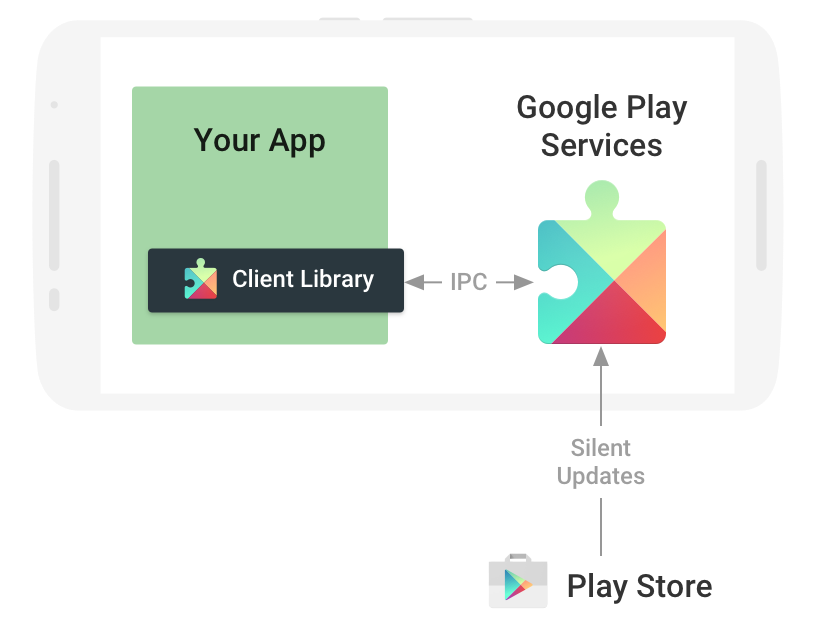
\includegraphics[width=\textwidth]{figures/play-services-diagram.png}
	\caption{Google Play Services communication\cite{GapiFigure}}
	\label{fig:gapifigure}
\end{figure}

\todo{Skal måske flyttes}
The Google play services have limits, and is not supporting devices with an Android version lower than 2.3. This means that the application will not be backwards compatible as we have chosen only to focus on devices of Andorid version 2.3 and newer.

As before mentioned the Google Play Service will allow the application to collect location data, but it is not doing so solely using the GPS in the device. The location service will use both the network and GPS to estimate a position as precise as possible\cite{GapiLocation}. To ensure the location data that is collected is relevant, it is needed to ensure the data is stored from when the user have been traveling by vehicle.
The Google Play Services have a service for this called Activity recognition. 

Activity recognition is a services which uses several sensors on the deices to determine what the user is currently doing. The service will return a serenity level from 1 to 100, where 100 is 100\% sure that a user is doing said activity.
The activity recognition will be used to ensure unnecessary data will be stored on the database. It may prevent some dirty data to be stored, that could be mistaken as routes from one location to another, which were not to be considered in this application in the first place. When a user is in a vehicle with a serenity level above 75\%\todo{placeholder}, data should be stored and used for computations.

The application must be running in the background while the device is on, for it to be able to differ between the users activity at all times and collect data. It is chosen only to  collect data point from the GPS every two minute\todo{placeholder}, while in a vehicle, to reduce load and improve battery life. Every data point collected during driving must be appended to a list that eventually will represent an entire route.

When the activity change from vehicle to any other activity the application will send the list with data points to the RideShare server, where it will take over the processing. 